%\documentstyle[epsf,twocolumn]{jarticle}       %LaTeX2.09�d�l
\documentclass[twocolumn]{jarticle} 
\setlength{\topmargin}{-45pt}
%\setlength{\oddsidemargin}{0cm} 
\setlength{\oddsidemargin}{-7.5mm}
%\setlength{\evensidemargin}{0cm} 
\setlength{\textheight}{24.1cm}
%setlength{\textheight}{25cm} 
\setlength{\textwidth}{17.4cm}
%\setlength{\textwidth}{172mm} 
\setlength{\columnsep}{11mm}

% 【節が変わるごとに (1.1)(1.2) … (2.1)(2.2) と数式番号をつけるとき】
%\makeatletter
%\renewcommand{\theequation}{%
%\thesection.\arabic{equation}} %\@addtoreset{equation}{section}
%\makeatother

%\renewcommand{\arraystretch}{0.95}行間の設定

%%%%%%%%%%%%%%%%%%%%%%%%%%%%%%%%%%%%%%%
\usepackage[dvipdfmx]{graphicx} %pLaTeX2e仕様(\documentstyle ->\documentclass)
\usepackage{url}		%参考文献にurlを入れる用
\usepackage{bm}  	%太字形式のベクトルを使う用
\usepackage{amsmath}	%数式の場合分け用
%%%%%%%%%%%%%%%%%%%%%%%%%%%%%%%%%%%%%%%

\begin{document}

	%bibtex用の設定
	%\bibliographystyle{ujarticle}

	\twocolumn[
		\noindent
		\hspace{1em}
		2021 年 5 月 14 日
		研究会資料
		\hfill
		B4	尾關  拓巳
		\vspace{2mm}
		\hrule
		\begin{center}
			{\Large \bf 進捗報告}
		\end{center}
		\hrule
		\vspace{9mm}
	]

\section{今週やったこと}
	\begin{itemize}
		\item CMA-ESの後にネルダーミード法をする最適化の実験
		\item ネルダーミード法の後にCMA-ESをする最適化の実装
	\end{itemize}

\section{CMA-ESの後にネルダーミード法をする最適化の実験}
	以下の2種類の実験をした.
	\begin{itemize}
		\item 実験1: CMA-ESを用いて最適化をし,制約違反を満たす最初の解をネルダーミード法の初期解として代入する.
		\item 実験2: CMA-ESを用いて最適化をし,最終世代の解をネルダーミード法の初期解として代入する.
	\end{itemize}
	\subsection{実験設定}
		表1に,実験1,2におけるネルダーミード法の実験設定を示す.
		\begin{table}[htbp]	%表1
			\begin{center}
				\caption{ネルダーミード法の実験設定}
				\begin{tabular}{| c | c |} \hline
					変化しない場合の許容回数 & 4000 \\
					変化とみなす閾値 & $10^{-11}$ \\ 
					最大操作数 & 無限 \\
					$\alpha$ & 1.0 \\
					$\gamma$ & 2.0 \\
					$\rho$ & 0.5 \\
					$\sigma$ & 0.5 \\ \hline
				\end{tabular}
			\end{center}
		\end{table}
		
		$\bm{x}$の初期位置は0から1のランダムな実数とする.

		\subsubsection{評価関数と制約違反}
			取り扱うベンチマーク問題では制約違反を考慮する必要があり,今実験ではその許容量を$1.0\times10^{-10}$とする.また,制約違反の合計値$V$を用いて式1のようにネルダーミード法の目的関数$F$を定義する.
			\begin{equation}	%式1
				F(\bm{x}) = \begin{cases}
					f(\bm{x}) & (V < 1.0\times10^{-10}) \\
					V + 10^7 & (otherwise)
				\end{cases}
			\end{equation}
			ただし,ベンチマークの目的関数を$f$とする.

		表2に,実験1,2におけるCMA-ESの実験設定を示す.
		\begin{table}[htbp] %表2
			\begin{center}
				\caption{CMA-ESの実験設定}
				\begin{tabular}{| c | c |} \hline
					最大世代数 & 6000 \\
					入力次元数 & 120 \\
					1世代あたりの個体数$\lambda$ & 1200 \\
					$\mu$ & 600 \\
					$\sigma^{(0)}$ & 0.05 \\ 
					$\bf{m}^{(0)}$ &  (5,...,5) \\ \hline
				\end{tabular}
			\end{center}
		\end{table}

	\subsection{実験1}
		図1に結果として得られた目的関数の推移を示す.縦軸は目的関数値,横軸は世代数または操作回数である.
		\begin{figure}	%図1
			\centering
            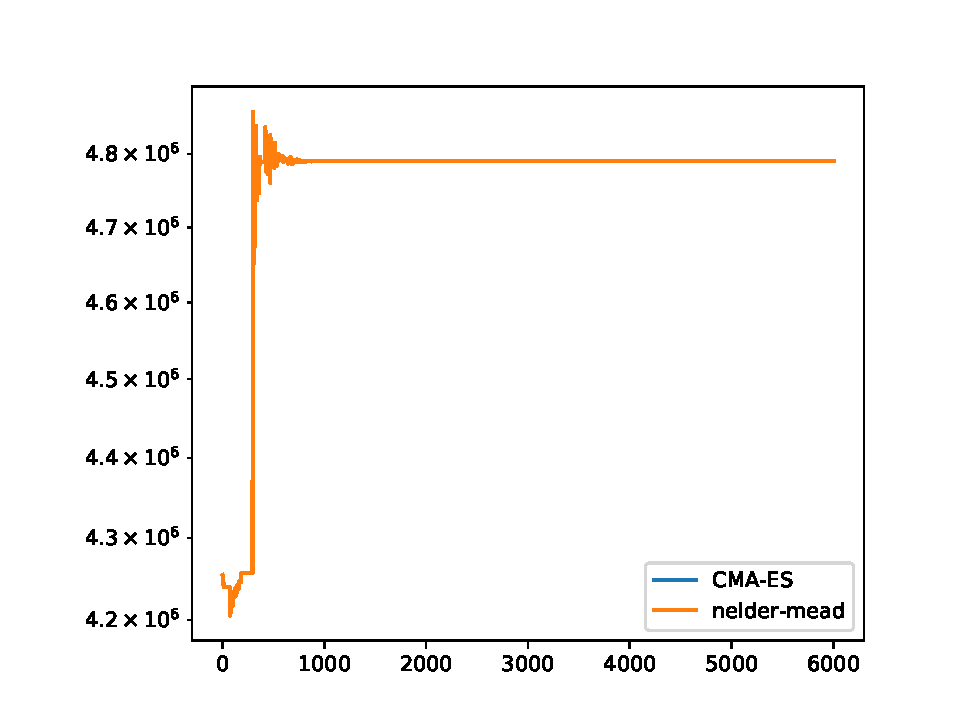
\includegraphics[width=9cm]{cmaes_nelder.pdf}
            \caption{目的関数値の推移}
        \end{figure}
		3005世代からネルダーミード法による最適化がされたが,図1を見る限りCMA-ESとネルダーミード法にはほとんど違いがない.ここで,図2に3005世代以降の目的関数値の推移を示す.縦軸は目的関数値,横軸は世代数または操作回数である.
		\begin{figure}	%図2
			\centering
            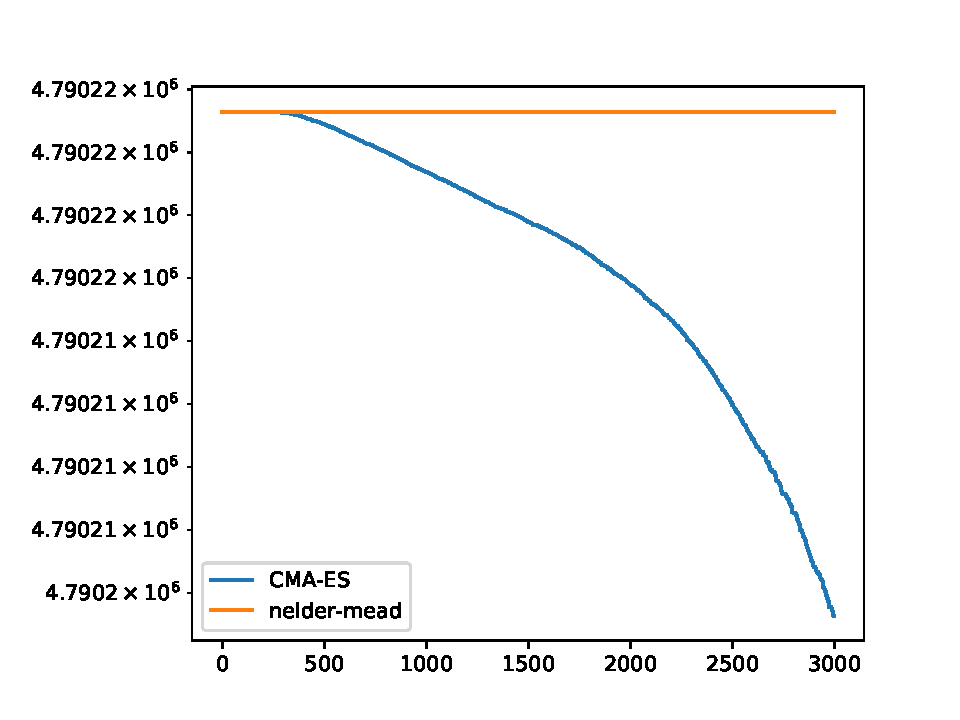
\includegraphics[width=9cm]{cmaes_nelder_v2.pdf}
            \caption{目的関数値の推移}
        \end{figure}
		図2より,CMA-ESの方がネルダーミード法より目的関数を最適化できていることがわかる.
	\subsection{実験2}
		図3に結果として得られた目的関数の推移を示す.縦軸は目的関数値,横軸は世代数と操作回数である.
		\begin{figure}	%図3
			\centering
            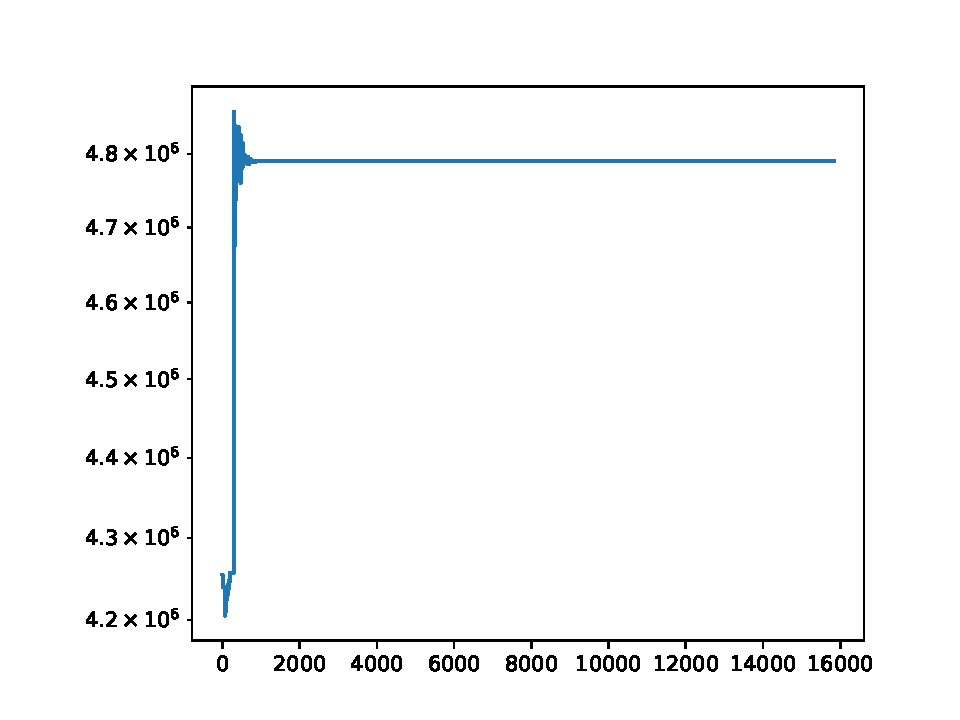
\includegraphics[width=9cm]{cmaes_nelder2.pdf}
            \caption{目的関数値の推移}
        \end{figure}
		図3より,CMA-ESの結果を用いたネルダーミード法は目的関数をほとんど最適化できていないことがわかる.

\section{ネルダーミード法の後にCMA-ESをする最適化の実装}
	上記と同様の設定でネルダーミード法からCMA-ESをする実装をした.ネルダーミード法における最後のλ回の試行から得られたλ個の$\bm{x}$をCMA-ESの初期個体群として代入した.図4に実装したコードでの目的関数値の推移を示す.縦軸は目的関数値,横軸は操作回数および世代数である.横軸の最後から6000世代がCMA-ESによる最適化である.
	\begin{figure}	%図4
		\centering
		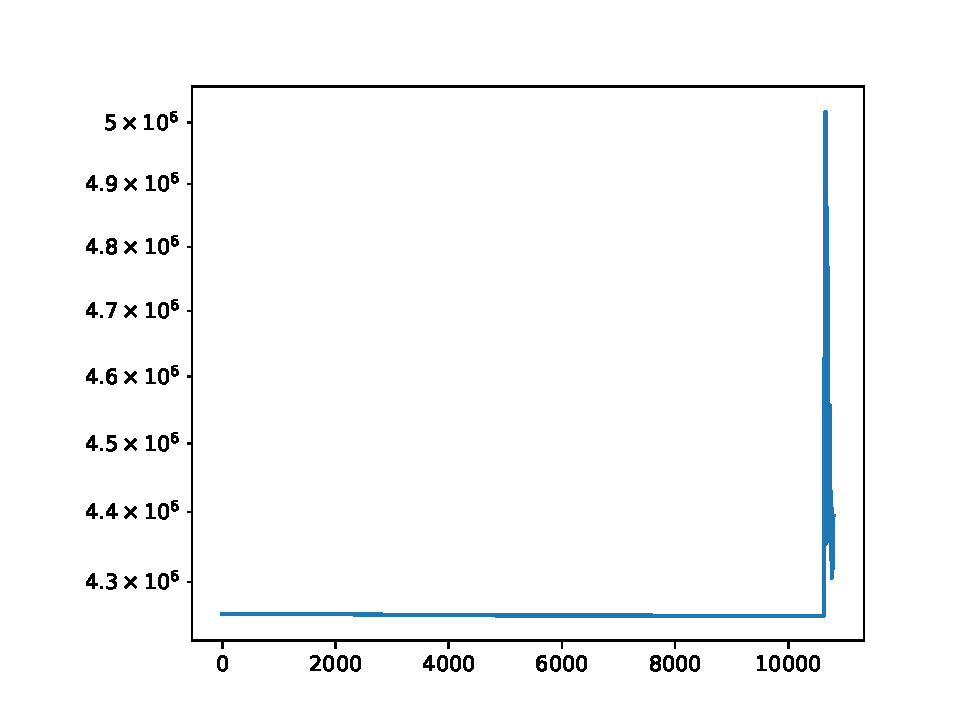
\includegraphics[width=9cm]{nelder_cmaes.pdf}
		\caption{目的関数値の推移}
	\end{figure}
	図4より,CMA-ESの前半,中盤がかなり停滞している.これはネルダーミード法から得た初期個体群の個体がほとんど似たような解であるためであると考えられる.
	
	CMA-ESの数世代ごとにネルダーミード法を挟むという手法も試してみたが,やはりネルダーミード法の後のCMA-ESの最適化がうまくいかなかった.
	ネルダーミード法から得るCMA-ESの初期個体群に何か工夫が必要であると考えた.
\section{CMA-ESの目的関数値と制約違反}
	図5,6にCMA-ESを用いたベンチマーク問題の最適化の目的関数値の推移と制約違反の合計値の推移を示す.図5の縦軸は目的関数値,図6の縦軸は制約違反の合計値,横軸は世代数である.制約違反の合計値は許容量以下となったら0としている.
	\begin{figure}	%図5
		\centering
		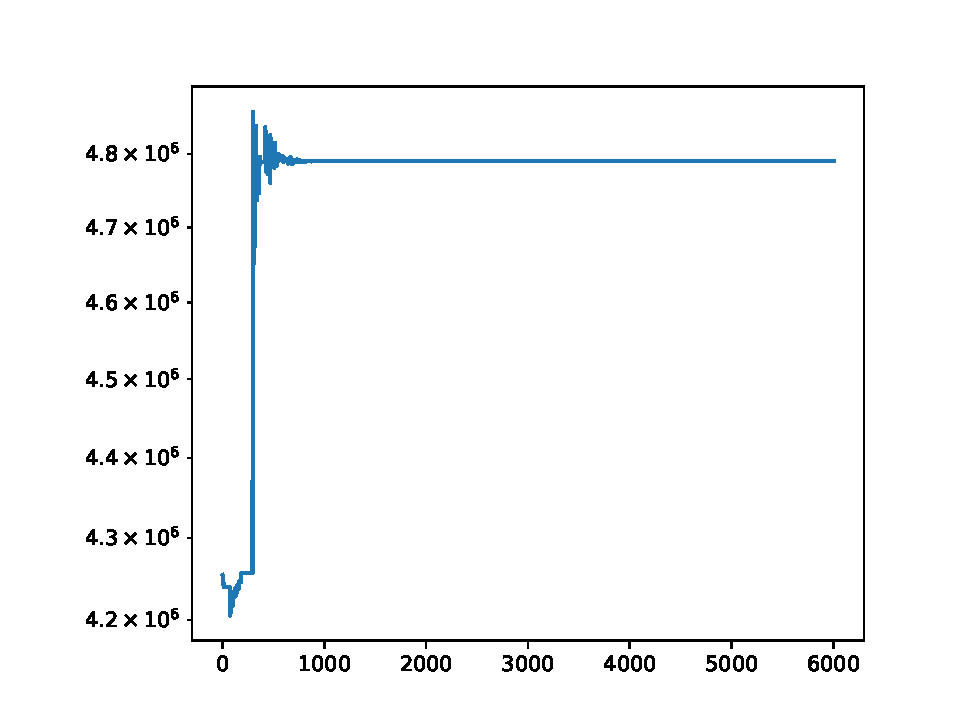
\includegraphics[width=9cm]{cmaes.pdf}
		\caption{目的関数値の推移}
	\end{figure}
	\begin{figure}	%図6
		\centering
		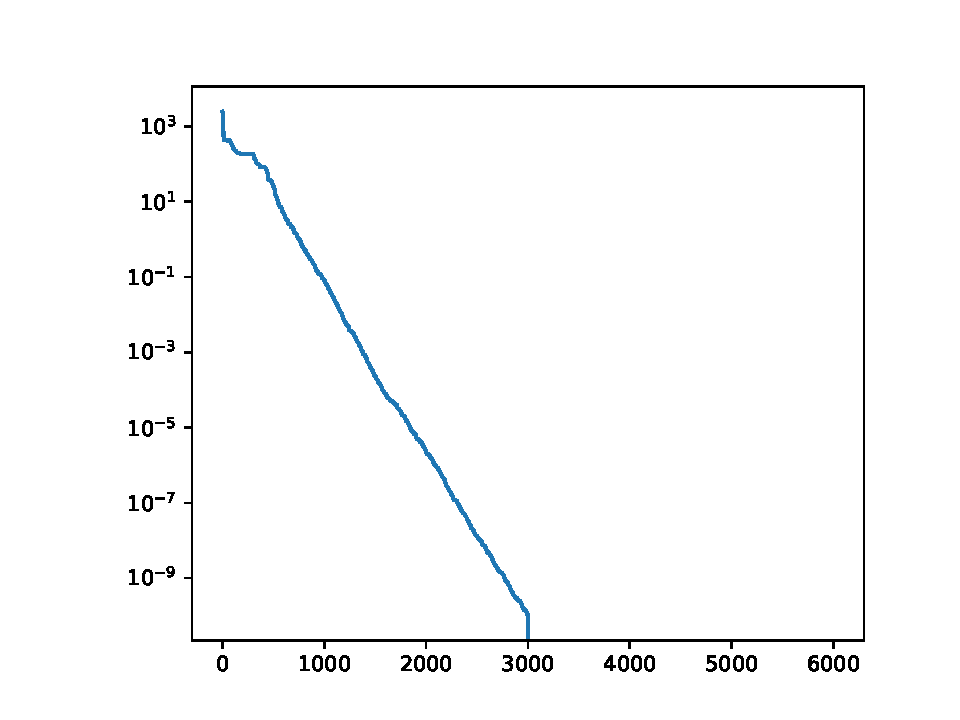
\includegraphics[width=9cm]{cmaes_V.pdf}
		\caption{制約違反の合計値の推移}
	\end{figure}

\section{今後の展望}
	CMA-ESを用いてベンチマーク問題の制約違反を優先して最適化をすると,目的関数値が約480万に落ち着いた.既存の見つかっている解の目的関数値が約400万であることを考えると,一つの局所解にたどり着き抜け出せなくなっている可能性が高い.したがって,ある程度制約違反を許しながら目的関数の最適化をするという方法が考えられる.

	さらにCMA-ESのパラメータの調整や,他のバリエーションのCMA-ESも用いてアプローチしたいと考えている.

% 参考文献
\bibliography{hoge}				%hogeはbibファイルのファイル名
\bibliographystyle{junsrt}		%順番に表示

\end{document}